\documentclass{article}

\usepackage{listings}
\usepackage[english]{babel}
\usepackage{color}
\usepackage{graphicx}
\graphicspath{{img/}}

\interlinepenalty 10000

\definecolor{dkgreen}{rgb}{0,0.6,0}
\definecolor{gray}{rgb}{0.5,0.5,0.5}
\definecolor{mauve}{rgb}{0.58,0,0.82}

\lstset{frame=tb,
  language=C++,
  aboveskip=3mm,
  belowskip=3mm,
  showstringspaces=false,
  columns=flexible,
  basicstyle={\small\ttfamily},
  numbers=none,
  numberstyle=\tiny\color{gray},
  keywordstyle=\color{blue},
  commentstyle=\color{dkgreen},
  stringstyle=\color{mauve},
  breaklines=true,
  breakatwhitespace=true,
  tabsize=3
}

\title{Spyke (Babel Project) - User's Guide}
\author{La Pintade}
\date{5 October 2015 - 8 November 2015}

\begin{document}

  \maketitle
  \tableofcontents

  \newpage

  \section{About}
  This document is a documentation for Users about Spyke. Spyke is a software developed by the La Pintade team. The team developed a Skype-like product in a month for the Epitech's Babel project.

  \bigskip
  This guide provides you a complete explanation over the Spyke program. However, if you want to go further and ask questions, please email us at info@spyke.com

  \newpage

  \section{Sign in}
  \bigskip
  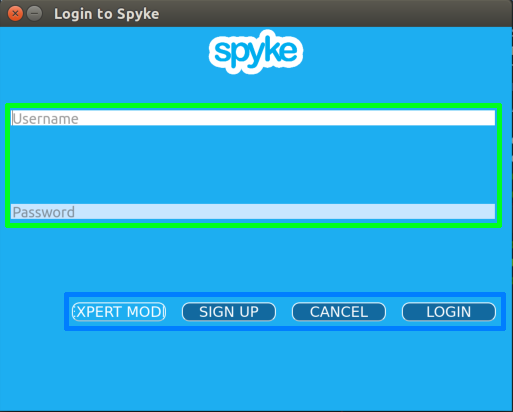
\includegraphics[width=350]{loginGuide}

  \bigskip
  You just launched Spyke ! This is the Login window.

  \bigskip
  In green, you can see the usual fields: Username and Password.

  \bigskip
  In blue, there are 4 buttons:

  Login: to validate your username / password. This opens the Home window.

  Cancel: to cancel your login. This closes Spyke.

  Sign Up: to register to Spyke. This opens the Signup window.

  Expert Mode: this allows you to chose the ip of the server you want to connect to. (Warning ! This is for expert, if you accidently changed the default value, just relaunch the program.)

  \newpage

  \section{Signup}
  \bigskip
  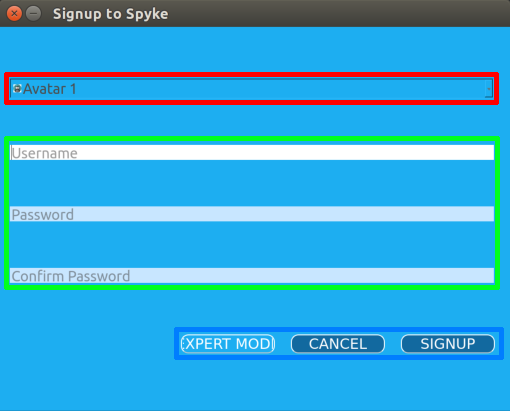
\includegraphics[width=350]{signupGuide}

  \bigskip
  This is the Signup window. You are here because you want to register to Spyke.

  \bigskip
  In red, you have a dropdown menu to chose between 8 avatars.

  \bigskip
  In green, the same fields that the Login window + the confirm password field.

  \bigskip
  In blue, there are 3 buttons:

  Login: to login to Spyke. This opens the Home window.

  Cancel: to cancel registering. This closes Spyke.

  Expert Mode: this allows you to chose the ip of the server you want to connect to. (Warning ! This is for expert, if you accidently changed the default value, just relaunch the program.)

  \newpage
  \section{Home}
  \bigskip
  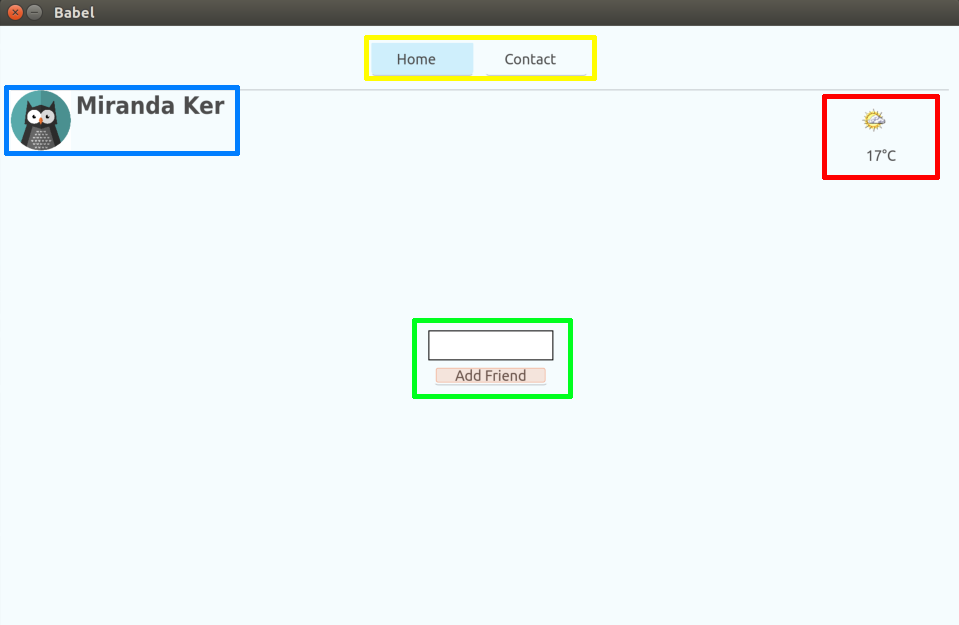
\includegraphics[width=350]{homeGuide}

  \bigskip
  This is the Home window. You are now logged into Spyke !

  \bigskip
  In blue, you have your Avatar and your login (chosen on signup).

  \bigskip
  In green, you have the field to add a contact: you can type here the login of the friend you want to add.

  \bigskip
  In red, you have the meteo of your city. (Go outside take some fresh air !)

  \bigskip
  Finally in yellow, you have 2 buttons to switch to the Contact window or the Home window.

  \newpage
  \section{Contact}
  \bigskip
  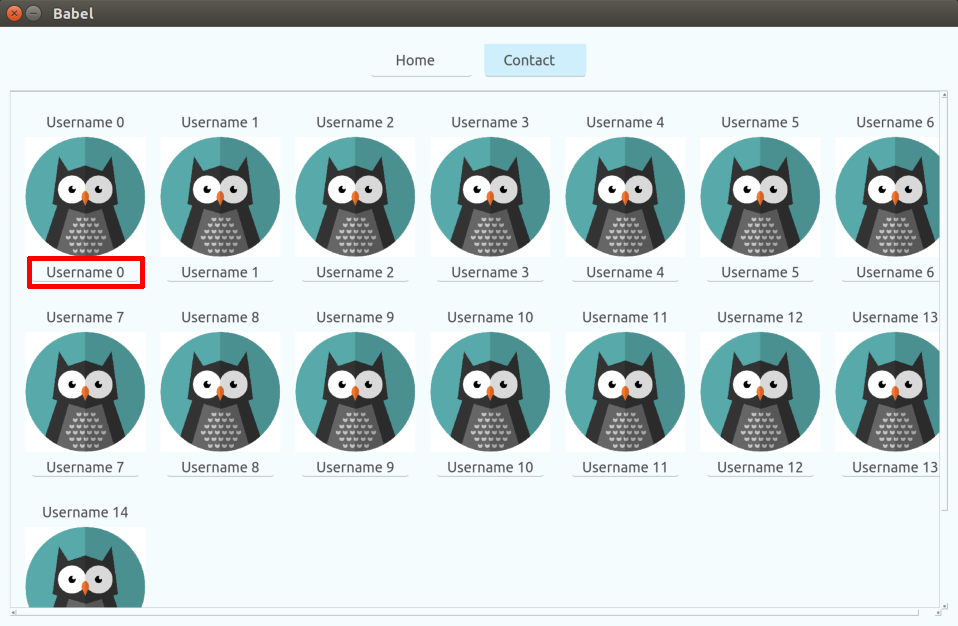
\includegraphics[width=350]{contactGuide}

  \bigskip
  This is the Contact window.

  \bigskip
  In this window, you can see every contact that you have.

  \bigskip
  In red, this is a button to access the Call window. You can have a Call window for every contact you have.

  \newpage
  \section{Call}
  \bigskip
  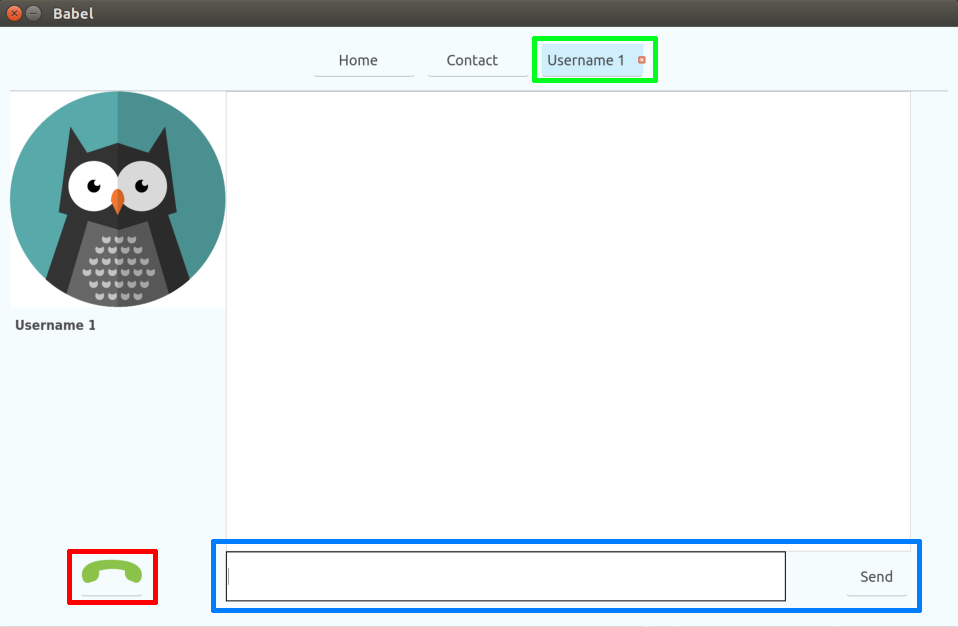
\includegraphics[width=350]{ownContactGuide}

  \bigskip
  This is the Call window.

  \bigskip
  In red, this is the button to Call your friend.

  \bigskip
  In blue, this is the field to chat with your contact. You can type your message and click on Send to send it.

  \bigskip
  In green, a new button appeared. This is the button to access the call window with your friend.

\end{document}
